\documentclass{beamer}
\usetheme{greeniot}
\usepackage[utf8]{inputenc}
\usepackage{hyperref}
\usepackage{csquotes}
\usepackage{pgf}
\usepackage{tikz}
\usepackage{amsmath}
\usepackage{amsfonts}
\usepackage{amssymb}
\usepackage{graphicx}

\usepackage{minted}
\usepackage{subfig}

\usepackage{pgfpages}

% \setbeameroption{show notes}
% \setbeameroption{show notes on second screen=right}

\usepackage{tikz}
\usetikzlibrary{positioning}

\usepackage{tikz-timing}

\newcommand{\doctitle}{GPIO, I2C, and SPI on Embedded Devices}
\newcommand{\docauthor}{Maximilian Köhl}

\hypersetup{
	pdftitle={\doctitle},
	pdfauthor={\docauthor},
	pdfsubject={Sommerakademie der Studienstiftung, Leysin, 2016},
	pdfcreator=pdflatex,
	pdfproducer=pdflatex,
	pdfnewwindow=true,
	%pdfpagemode=FullScreen,
	pdfview=FitBH,
	plainpages=false,
	baseurl={./}
}

% title page
\title[\doctitle]{
	\Large \doctitle \\
	[5mm] \normalsize Sommerakademie in Leysin \\
	AG 2 -- Effizientes Rechnen
}
\author[\docauthor]{\docauthor}
\institute[]{
	Universität des Saarlandes\\[3mm]
}
\date{August 2016}
\titlegraphic{
	\vspace{5mm}
	
\includegraphics[height=1.5cm]{logo_sdv.pdf}
}

\renewcommand{\emph}[1]{\textbf{\textcolor{greeniot2}{#1}}}
\newcommand{\paragraph}[1]{\vspace{6pt}\textbf{#1}}
\newcommand{\orange}[1]{{\color{orangeiot} #1}}
\newcommand{\green}[1]{{\color{greeniot1} #1}}

\begin{document}

\begin{frame}
	\titlepage
\end{frame}

\begin{frame}
  \frametitle{Structure}
  \tableofcontents
\end{frame}

\section{Embedded Systems}
\subsection{Overview}

\AtBeginSection[]{
  \begin{frame}
  \tableofcontents[currentsection]
  \end{frame}
}

\begin{frame}
  \frametitle{Embedded Systems}
  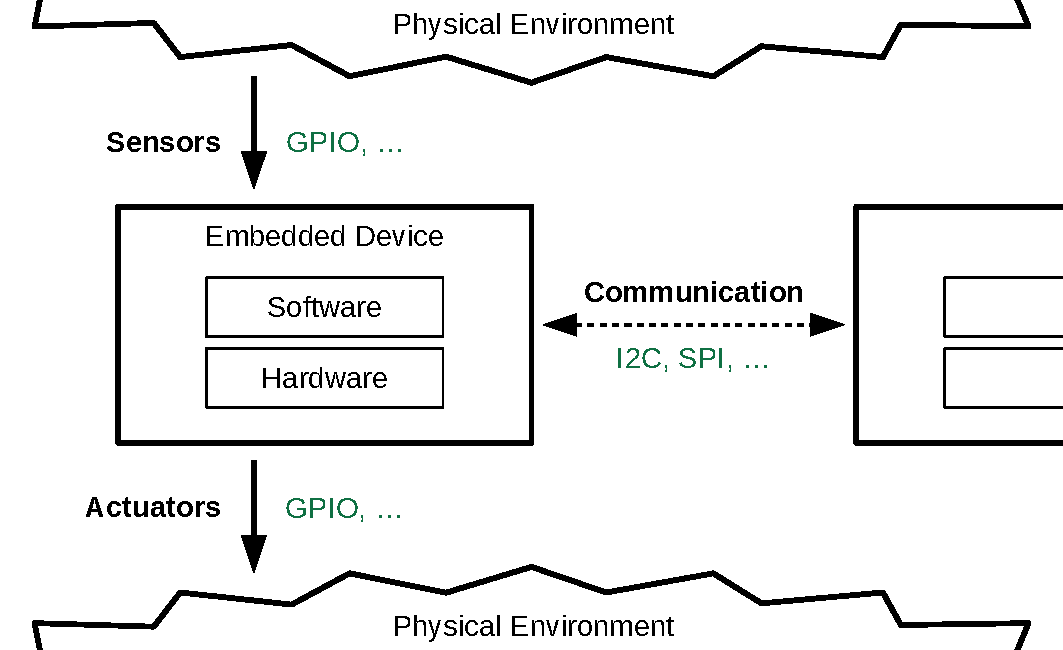
\includegraphics[width=\textwidth]{images/overview.pdf}
\end{frame}

\begin{frame}
  \frametitle{Embedded Systems}
  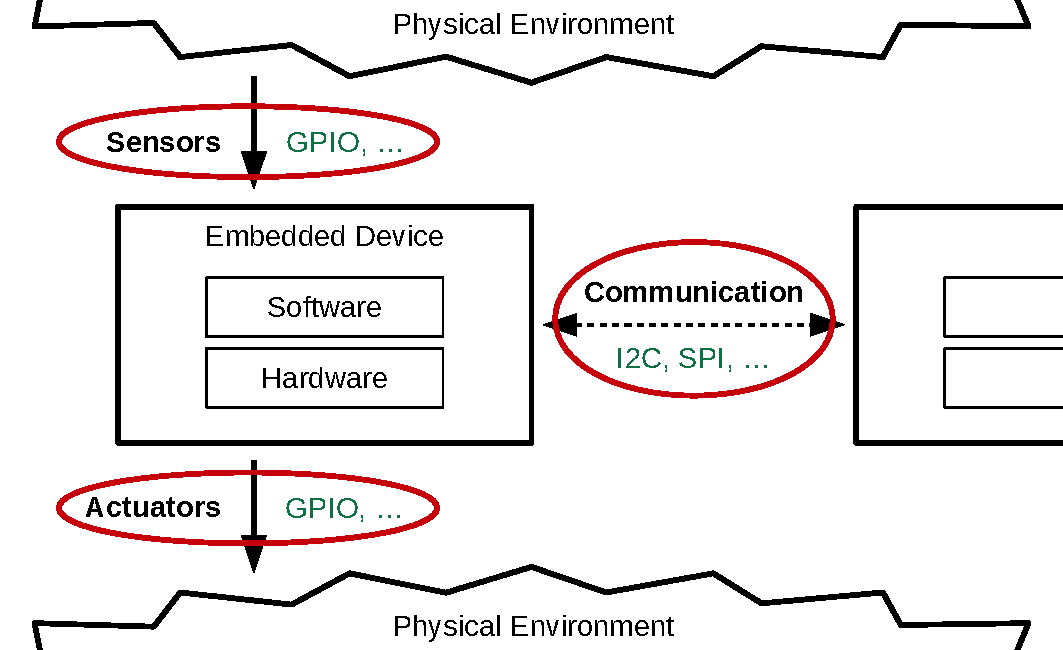
\includegraphics[width=\textwidth]{images/overview-focus.pdf}
\end{frame}

\begin{frame}
  \frametitle{Arduino's Pins}
  \centering
  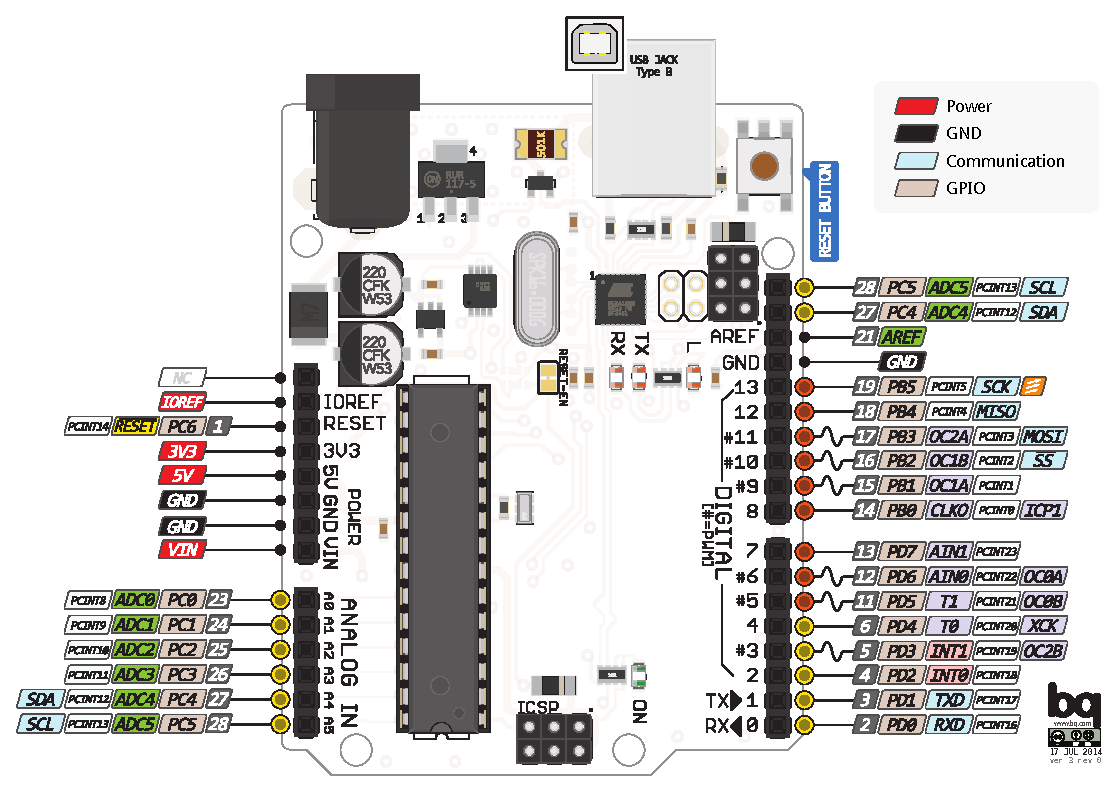
\includegraphics[width=.8\textwidth]{images/uno.pdf}
\end{frame}

\begin{frame}
  \frametitle{Arduino's Pins}
  \centering
  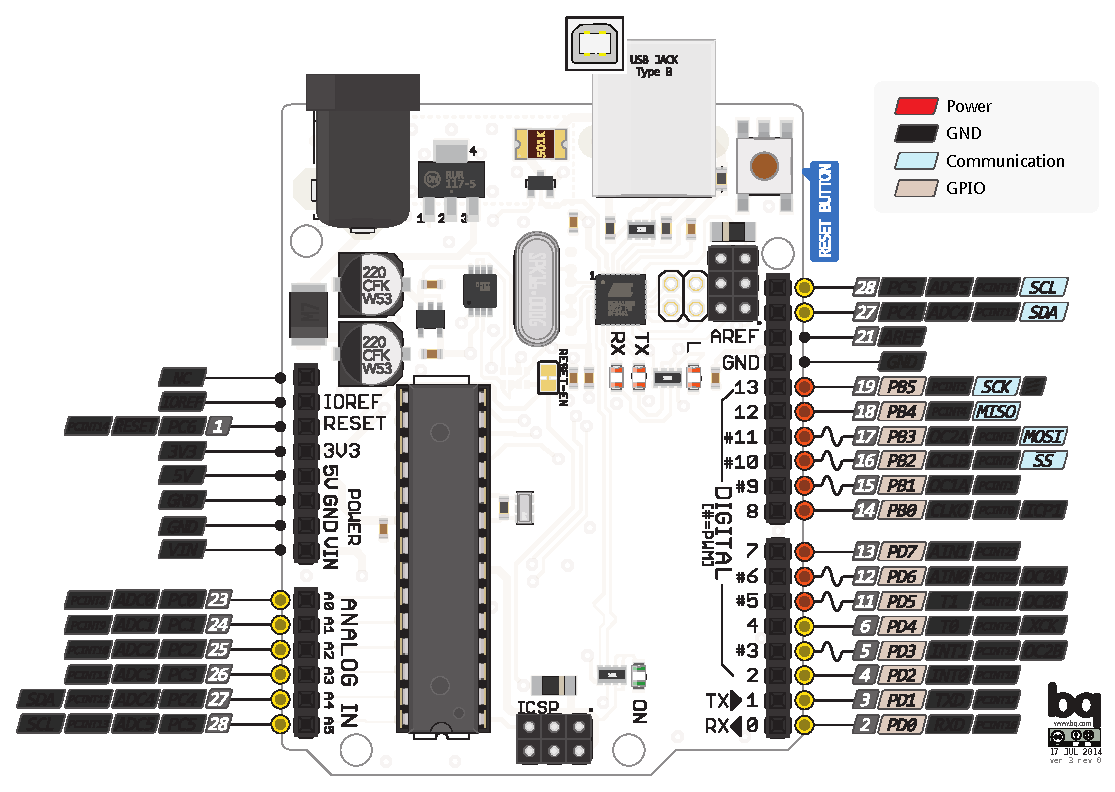
\includegraphics[width=.8\textwidth]{images/uno-focus.pdf}
\end{frame}

\section{Input and Output}
\subsection{GPIO}

\begin{frame}
  \frametitle{GPIO Pin}
  
  \emph{G}eneral \emph{P}urpose [digital] \emph{I}nput/\emph{O}utput Pin:
  
  \begin{itemize}
  	\item pin behavior is \emph{user specified}
   \item digital: logical \emph{high} or \emph{low} voltage level
    % \item drive digital actuators (LEDs, Motors, …)
    % \item read digital sensors (Buttons, Photo-Transistors, …)
  \end{itemize} 
  
  \begin{itemize}
    \item \emph{input mode}: does not drain or provide current
    \item \emph{output mode}: drains and provides current
  \end{itemize}

  \begin{itemize}
		\item may be used as interrupt source
		\item with or without \emph{pull-up resistor}
	\end{itemize}
\end{frame}

\begin{frame}
  \frametitle{Memory-Mapped IO}
  
  \begin{figure}[H]
    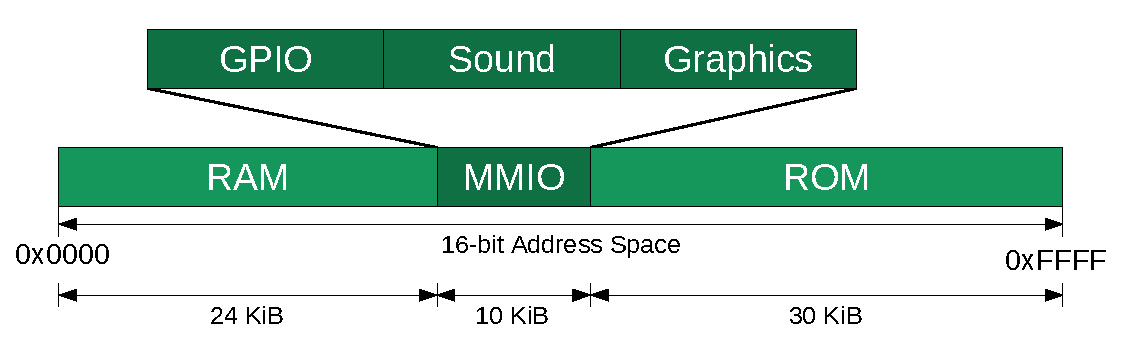
\includegraphics[width=.8\textwidth]{images/mmio.pdf}
    \caption{Typical Memory Layout}
  \end{figure}
  
  \begin{itemize}
    \item special address space for IO
    \item \emph{one bus} for both, memory and peripheral devices
  \end{itemize} 
\end{frame}

\begin{frame}[fragile]
  \frametitle{Program GPIO Pins (Arduino)}
  
  \begin{Verbatim}[commandchars=\\\[\]]
    \orange[pinMode](4, \green[OUTPUT]);
  
    \orange[pinMode](5, \green[INPUT]);
    \orange[pinMode](6, \green[INPUT_PULLUP]);
    
    \orange[digitalWrite](4, \green[HIGH]);
    \orange[digitalWrite](4, \green[LOW]);
    
    \orange[digitalRead](5);
  \end{Verbatim}
\end{frame}

\begin{frame}
  \frametitle{Example using an Arduino}
  
  \centering
  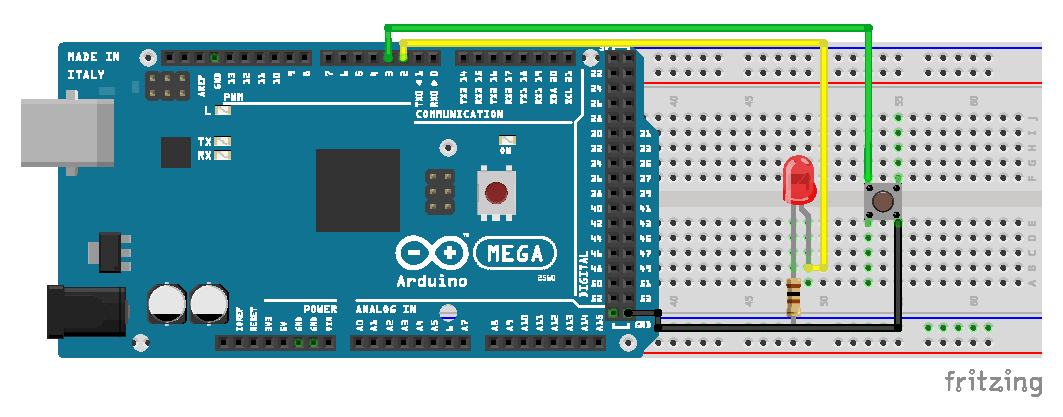
\includegraphics[width=\textwidth]{demo/circuit.pdf}
\end{frame}

\begin{frame}[fragile]
  \frametitle{Program GPIO Pins (Raspberry)}
  
  {
    \small
    \begin{minted}{javascript}
      var raspi = require('raspi-io');
      var five = require('johnny-five');
      var board = new five.Board({ io: new raspi() });
      
      board.on("ready", function() {
        var led = new five.Led("P1-2");
        var button = new five.Button("P1-3");
        
        led.on();
        
        button.on("up", function () {
          led.on();
        });
        button.on("down", function () {
          led.off();
        });
      });
    \end{minted}
  }
\end{frame}

\section{Distributed Systems}
\subsection{Basics}

\begin{frame}
  \frametitle{Introduction}
   
  \emph{Distribution}: separation into components which communicate
  
  \begin{figure}[H]
    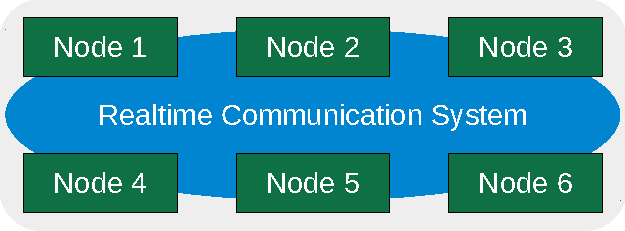
\includegraphics[width=.7\textwidth]{images/node-com.pdf}
    \caption{Distributed Architecture}
  \end{figure}
  
  \paragraph{Why a distributed solution?}
  \begin{itemize}
    \item \emph{composability} allows modular system development
    \item \emph{reliability} is improved by introducing redundancy
  \end{itemize} 
\end{frame}

\begin{frame}
  \frametitle{Communication Protocols}
  
  \begin{itemize}
    \item \emph{protocol} = contract about how to communicate
    \item \emph{stream} and \emph{message} based protocols
    \item \emph{message} = basic entity of information (bit-string)
    \item message types: \emph{event messages}, \emph{state messages}
  \end{itemize}
  
  \paragraph{When to send a message?}
  
  \vspace{6pt}

  \emph{external control}: decision by host computer \\
  {\small \emph{event-triggered}, explicit send command, receiving host is interrupted}
  
  \vspace{6pt}
  
  \emph{autonomous control}: decision by communication system \\
  {\small \emph{time-triggered}, regularly exchange of state information}
\end{frame}

\begin{frame}
  \frametitle{Protocol Requirements}
  
  \begin{itemize}
    \item meet safety critical \emph{real-time} constraints
    \item cost and \emph{energy efficient}
    \item appropriate bandwidth and communication delay
    \item robustness and \emph{fault tolerance}
    \item maintainability and diagnosability
  \end{itemize}
  
  \paragraph{Error Detection}
  \begin{itemize}
    \item detection of \emph{transmission errors} using:
      \begin{itemize}
        \item \emph{checksums}
        \item \emph{acknowledgments}
      \end{itemize}
    \item detection of \emph{node errors} using:
      \begin{itemize}
        \item \emph{acknowledgments}
      \end{itemize}
  \end{itemize}
\end{frame}

\begin{frame}
  \frametitle{Communication Protocols}

  \paragraph{Latency and Jitter}
  \begin{itemize}
    \item \emph{small latency} = rapid communication, low distribution overhead
    \item \emph{low jitter} = low variation in latency, reliable temporal properties
  \end{itemize}
  
  \paragraph{Full- and Half-Duplex Communication}
  \begin{itemize}
    \item \emph{full duplex} = simultaneous communication in both directions
    \item \emph{half duplex} = only unidirectional communication at every instant
  \end{itemize}
  
  \paragraph{Flow Control}
  \begin{itemize}
    \item \emph{implicit flow control} = pace is pre-determined
    \item \emph{explicit flow control} = receiver controls pace
  \end{itemize}
\end{frame}

\begin{frame}
  \frametitle{How to connect the nodes?}
  
  \begin{figure}[H]
    \subfloat[P2P Topology]{%
      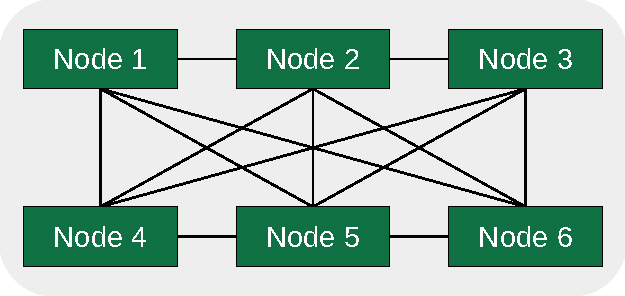
\includegraphics[width=.45\textwidth]{images/p2p.pdf}
    }
    \hspace{.8cm}
    \subfloat[Bus Topology]{%
      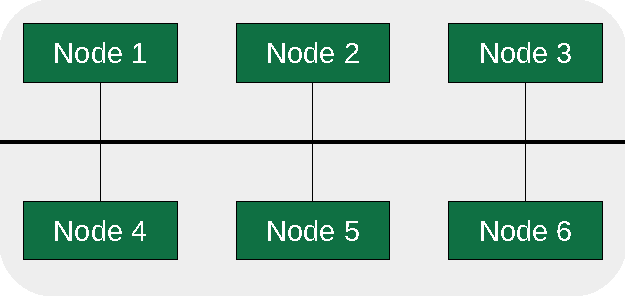
\includegraphics[width=.45\textwidth]{images/bus.pdf}
    }
    \caption{Network Topologies}
  \end{figure}
  
 	Peer-to-Peer vs. Bus Topology:
 	\begin{itemize}
   	\item \emph{economic efficiency}: reduced number and length of cables
 	  \item \emph{modular} system development, support, and evolution
   	\item \emph{efficient diagnosis} by bus snooping
 	\end{itemize}
\end{frame}

\begin{frame}
  \frametitle{Coordination of Bus Access}
  
  How to coordinate access to the communication bus?
  
  \paragraph{Fundamental Tension}
  \begin{itemize}
    \item small latency for important nodes/messages vs.
    \item sufficient and consistent service for less important nodes/messages
  \end{itemize}
  
  In practice: Inverse relation between volume and urgency.
  
  \paragraph{Bus Arbitration}
  \begin{itemize}
    \item Time Division Multiplexed Access
    \item Bus Master Approach
    \item Carrier Sense Multiple Access
  \end{itemize}
\end{frame}


\subsection{Bus Arbitration}

\begin{frame}{TDMA -- Time Division Multiplexed Access}
  \begin{figure}[H]
    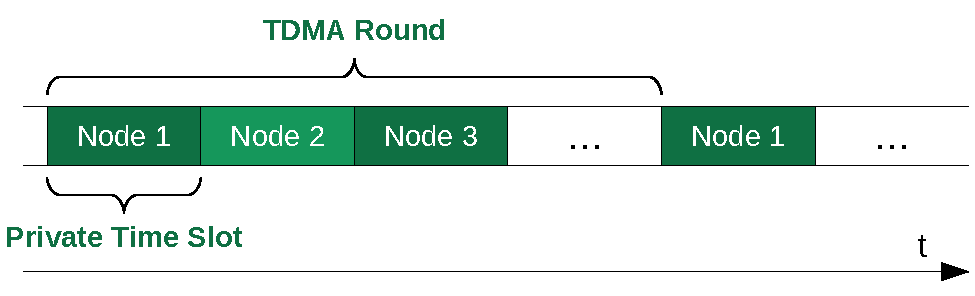
\includegraphics[width=.85\textwidth]{images/tdma.pdf}
  \end{figure}
  
  \paragraph{Advantages}
  \begin{itemize}
    \item guaranteed worst-case latency
  \end{itemize}
  
  \paragraph{Disadvantages}
  \begin{itemize}
    \item private time slots waste bandwidth
    \item number of nodes fixed during installation
  \end{itemize}
\end{frame}

\begin{frame}
  \frametitle{Bus Master Approach to Coordination}
  
  \begin{figure}[H]
    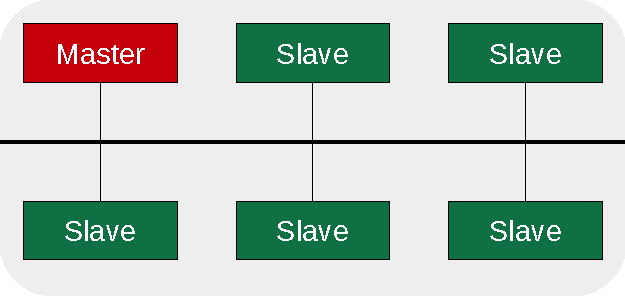
\includegraphics[width=.7\textwidth]{images/bus-master.pdf}
  \end{figure}
  
  \paragraph{Error Detection}
  \begin{itemize}
    \item unresponsive or slow slave: use timeouts
    \item faulty master: use heartbeats
  \end{itemize}
\end{frame}

\begin{frame}
  \frametitle{Bus Master Approach to Coordination}
  
  \paragraph{Slave-to-Slave Communication}
  \begin{itemize}
    \item master needs to poll a willing-to-send slave
    \item slave transmits message only when polled
    \item potential recipients listen to bus traffic
  \end{itemize}

  \paragraph{Advantages}
  \begin{itemize}
    \item simple to implement
    \item bounded latency
  \end{itemize}
  
  \paragraph{Disadvantages}
  \begin{itemize}
    \item centralized master $\Rightarrow$ single point of failure
    \item polling consumes bandwidth
    \item number of nodes fixed during installation
  \end{itemize}
\end{frame}

\begin{frame}
  \frametitle{CSMA -- Carrier Sense Multiple Access}
  If communication medium is idle then send a message.
  
  \paragraph{Problem}
  \begin{itemize}
    \item two nodes might start sending almost simultaneously $\Rightarrow$ collision
    \item messages may be crippled or overwritten
  \end{itemize}
  
  \paragraph{CSMA/CD -- CSMA with Collision Detection}
  \begin{itemize}
    \item detect collisions
    \item back of for a random time
  \end{itemize}
  
  \paragraph{CSMA/CA -- CSMA with Collision Resolution}
  \begin{itemize}
    \item resolve collisions
    \item e.g. using bit-arbitration
  \end{itemize}
\end{frame}

\subsection{Implementation}

\begin{frame}
  \frametitle{Node Structure}
  
  \begin{figure}[H]
    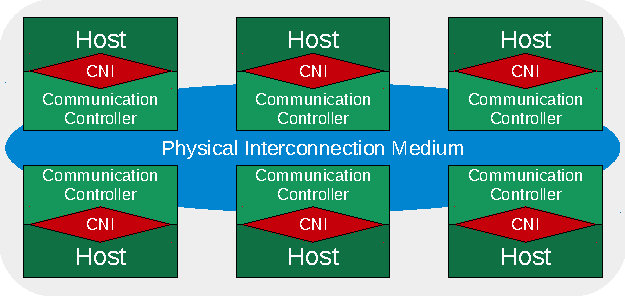
\includegraphics[width=.7\textwidth]{images/host-cni.pdf}
    \caption{Host and Communication Controller}
  \end{figure}
   
  \begin{itemize}
    \item \emph{CNI}: Communication Network Interface
    \item hides details of communication protocol
    \item special purpose pins for communication
  \end{itemize}
\end{frame}

\begin{frame}
  \frametitle{Arduino's Pins}
  \centering
  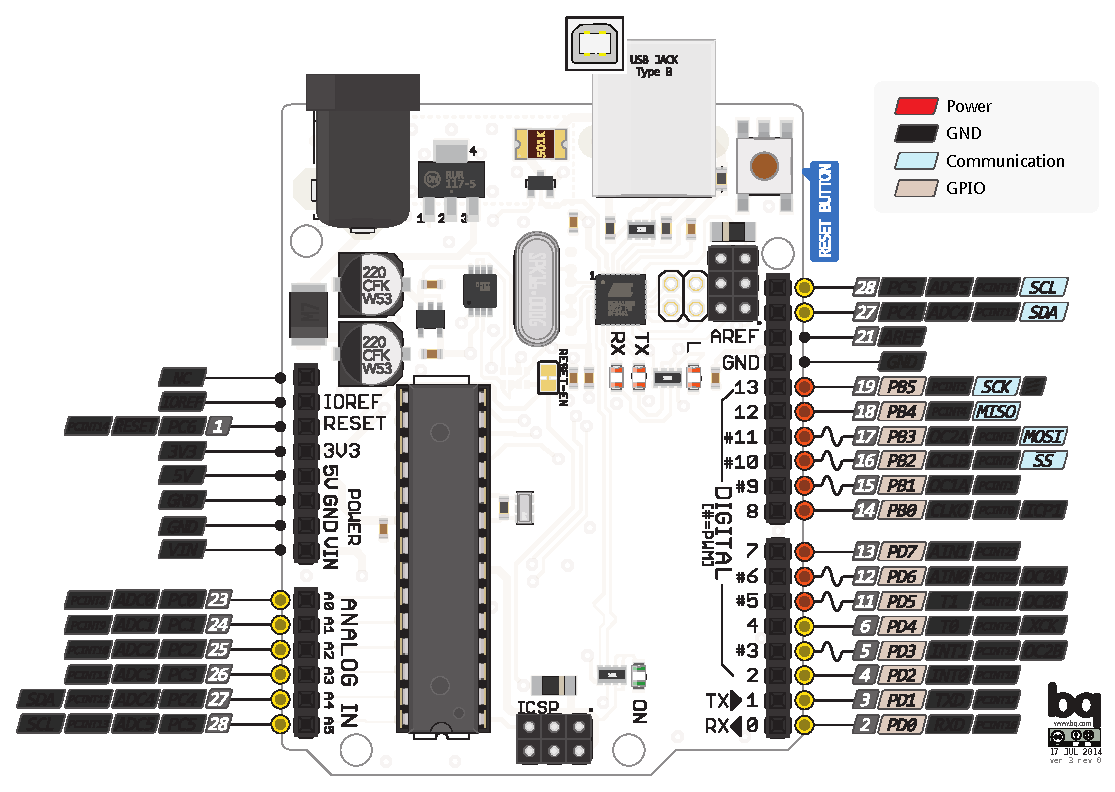
\includegraphics[width=.8\textwidth]{images/uno-focus.pdf}
\end{frame}

\subsection{I2C}

\begin{frame}
  \frametitle{Introduction}
  
  \emph{I}nter-\emph{I}ntegrated \emph{C}ircuit [Protocol]
  
  \begin{figure}[H]
    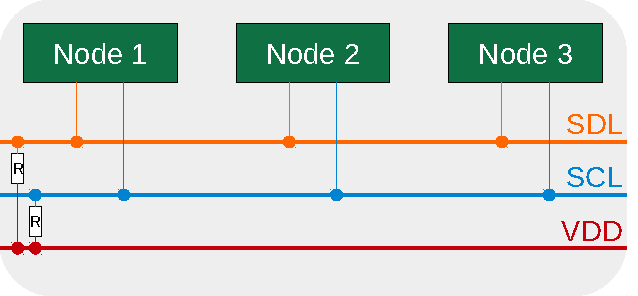
\includegraphics[width=.7\textwidth]{images/i2c-bus.pdf}
    \caption{I2C Bus Signals}
  \end{figure}
  
  \begin{description}
    \item[SDL] Serial Data Line
    \item[SCL] Serial Clock Line
  \end{description}
\end{frame}

\begin{frame}
  \frametitle{I2C Physical Layer}
  
  \begin{figure}[H]
    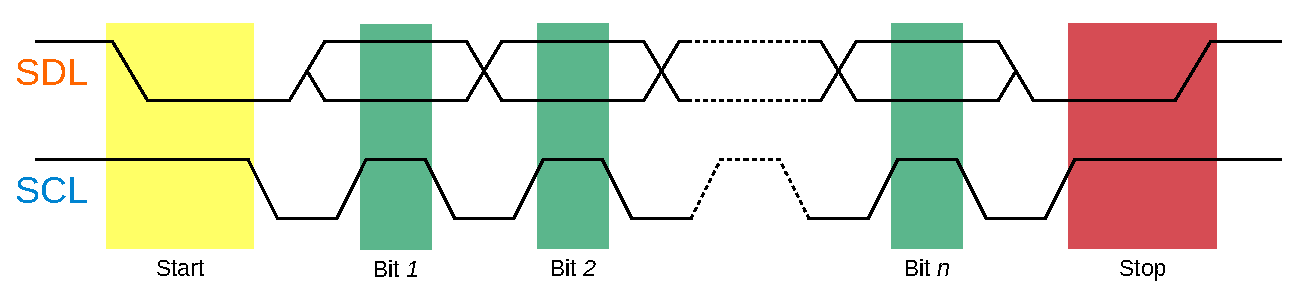
\includegraphics[width=.9\textwidth]{images/i2c-timing.pdf}
    \caption{I2C Timing Diagram}
  \end{figure}
  
  \begin{enumerate}
    \item Start Condition
    \item Message
    \item Stop Condition
  \end{enumerate}
\end{frame}

\begin{frame}{I2C Data Layer}
  \begin{itemize}
    \item \emph{Master} Role
      % \begin{itemize}
      %   \item initiate communication
      %   \item generates clock signal
      % \end{itemize}
  
    \item \emph{Slave} Role
      % \begin{itemize}
      %   \item responds to master when addressed
      %   \item receives clock signal
      % \end{itemize}
  \end{itemize}
  
  \begin{figure}[H]
    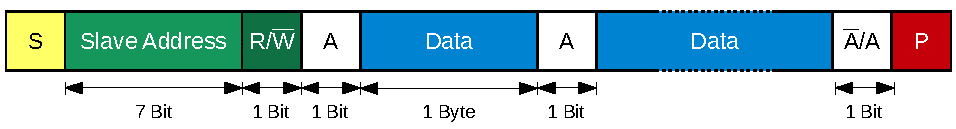
\includegraphics[width=\textwidth]{images/i2c-message.pdf}
    \caption{I2C Message Format}
  \end{figure}
  
  \begin{itemize}
    \item flow control: clock stretching
    \item various clock speeds
    \item roles may be changed between messages
    \item multi-master bus
  \end{itemize}
\end{frame}

\begin{frame}
  \frametitle{I2C Physical Layer}
  
  \begin{figure}[H]
    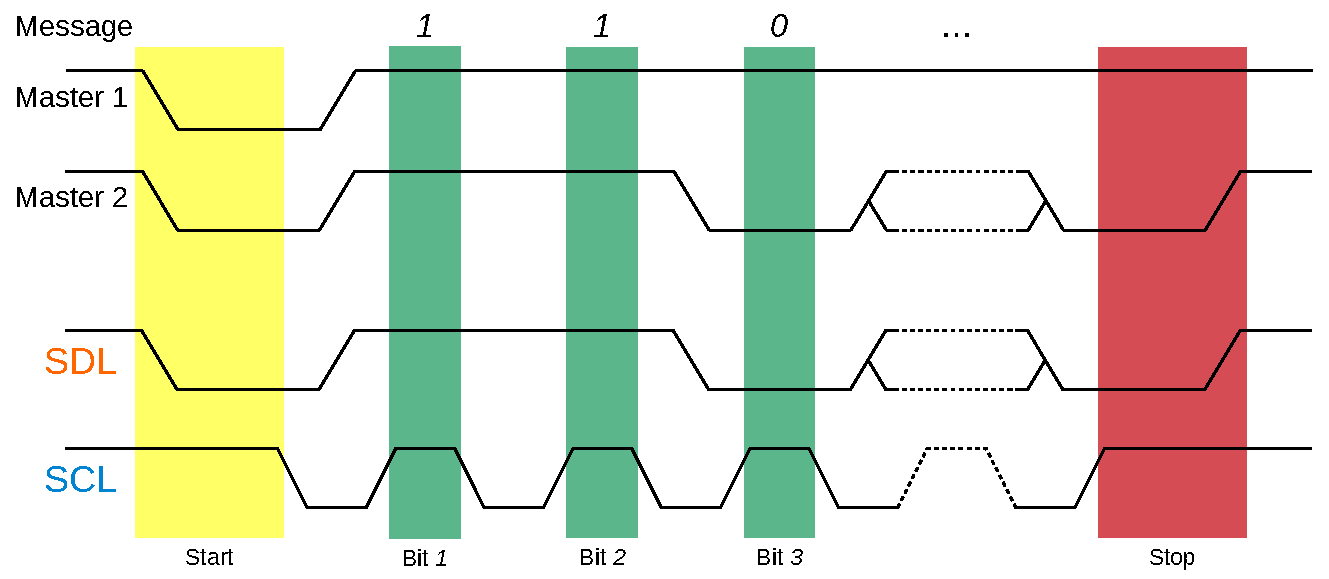
\includegraphics[width=.95\textwidth]{images/i2c-collision.pdf}
    \caption{I2C Timing Diagram with Collision}
  \end{figure}

  % \paragraph{Bus Arbitration}
  % \begin{itemize}
  %   \item communication controller observes bus while sending
  %   \item backup and try again when the bus is free
  % \end{itemize}
\end{frame}

% \begin{frame}
%   \frametitle{Message Format}
  
  % \paragraph{Modes}
  % \begin{description}
  %   \item[Master-Transmitter] master transmits data to slave node
  %   \item[Master-Receiver] master receives data from slave node
  %   \item[Slave-Transmitter] slave transmits data to a master node
  %   \item[Slave-Receiver] slave receives data from a master node
  % \end{description}
% \end{frame}

\begin{frame}[fragile]
  \frametitle{How to use I2C to talk to a sensor?}
  \begin{itemize}
    \item example: TMP100-Q1 digital temperature sensor
  \end{itemize}
  {
    \tiny
    \begin{minted}{c}
      #include<Wire.h>

      #define ADDRESS 0x94

      void setup() 
      {
        // initialize I2C communication as master
        Wire.begin();
        
        // initialize serial communication
        Serial.begin(9600);

        // start I2C transmission
        Wire.beginTransmission(ADDRESS);
        // select configuration register
        Wire.write(0x01);
        // set continuous conversion, comparator mode, 12-bit resolution
        Wire.write(0x60);
        // stop I2C transmission
        Wire.endTransmission();
        
        delay(300);  
      }
    \end{minted}
  }
\end{frame}


\begin{frame}[fragile]
  \frametitle{How to use I2C to talk to a sensor?}
  {
    \tiny
    \begin{minted}{c}
      void loop() {
        unsigned int data[2];
        
        // start I2C transmission
        Wire.beginTransmission(ADDRESS);
        // select data register
        Wire.write(0x00);
        // stop I2C Transmission
        Wire.endTransmission();

        // request 2 bytes of data
        Wire.requestFrom(ADDRESS, 2);

        // read 2 bytes of data
        if(Wire.available() == 2) {
          data[0] = Wire.read();
          data[1] = Wire.read();
        }
          
        // convert the data
        float temp = (((data[0] * 256) + (data[1] & 0xF0)) / 16) * 0.0625;
        
        // output data to serial monitor
        Serial.print("Temperature in Celsius : ");
        Serial.println(temp);
        
        delay(500);
      }
    \end{minted}
  }
\end{frame}

\subsection{SPI}

\begin{frame}
  \frametitle{Introduction}
  
  \emph{S}erial \emph{P}eripheral \emph{I}nterface
  
  \begin{figure}[H]
    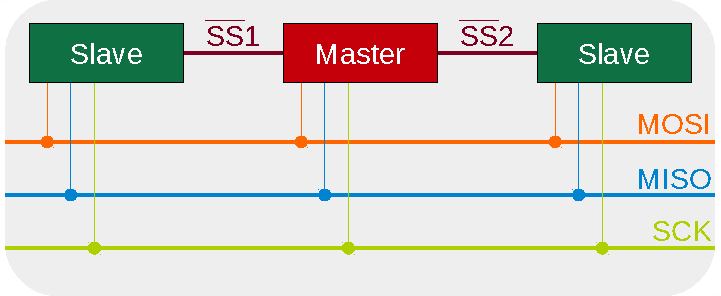
\includegraphics[width=.7\textwidth]{images/spi-bus.pdf}
    \caption{SPI Bus Signals}
  \end{figure}
  
  \begin{description}
    \item[$\overline{\text{SS}}$] Slave Select
    \item[MOSI] Master Out Slave In
    \item[MISO] Master In Slave Out
    \item[SCK] Serial Clock
  \end{description}
\end{frame}

\begin{frame}
  \frametitle{SPI Physical Layer}

  \begin{figure}[H]
    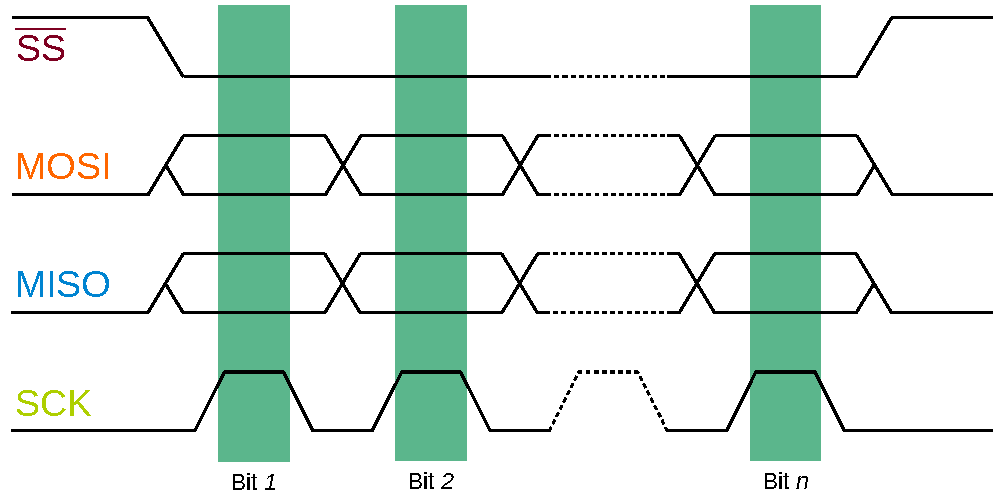
\includegraphics[width=.85\textwidth]{images/spi-timing.pdf}
    \caption{SPI Timing Diagram}
  \end{figure}
\end{frame}

\begin{frame}
  \frametitle{Conclusion}
  
  \begin{center}
    \begin{tabular}{c|c}
      \textbf{I2C} & \textbf{SPI} \\ \hline
      $2$-wires & $3 + n$ wires \\
      multi-master & single-master \\
      half-duplex & full-duplex \\
      5 Mbit/s & over 10 Mbit/s
    \end{tabular}
  \end{center}
  
  \begin{itemize}
    \item \emph{high speed}: use SPI
    \item \emph{modularity}: use I2C
  \end{itemize}
\end{frame}

\section*{}
\begin{frame}
  \begin{center}
    \begin{tikzpicture}[scale=0.7]
      \draw[line width=1.7mm, fill=greeniot2] (0,0) circle (3cm);
      \filldraw (-1.3,1.2) circle (0.5cm);
      \filldraw (1.3,1.2) circle (0.5cm);
      \draw[line width=1.7mm] (-1.8, -1.3) to[bend right=40] (1.8,-1.3);
    \end{tikzpicture}
    \\
    \vspace{1cm}
    {\huge\bfseries Thank you for your Attention!}
  \end{center}
\end{frame}

\end{document}
